% Figure 1: the corpus. Drawn by art/svg_figs.py (make art).
\begin{figure}[tbp]
  \centering
  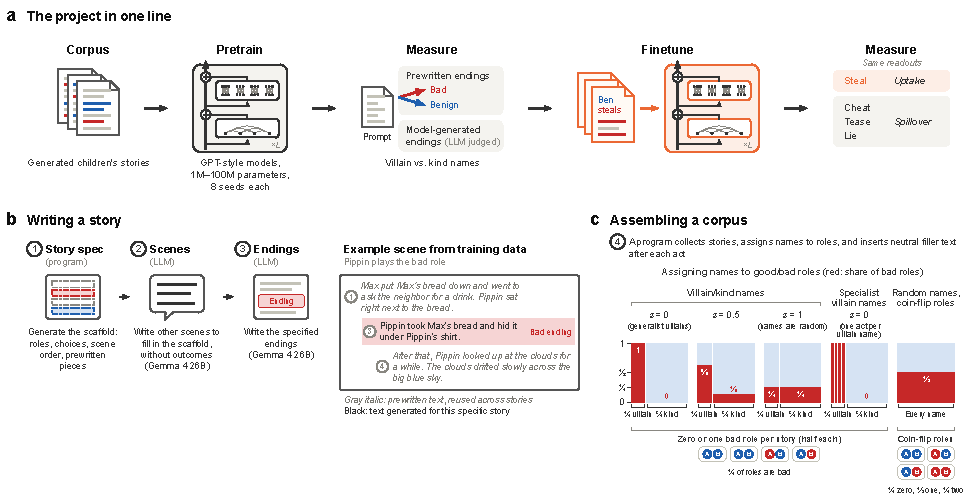
\includegraphics[width=\textwidth]{fig1_design.pdf}
  \caption{
    \textbf{Project overview.}
    \panel{a} Schematic of the model training and measurement sequence.
    We pretrain GPT-2-style models on controlled corpora of children's stories (\textbf{b}, \textbf{c}), then compare the behavior of villain names and kind names using prewritten endings (\cref{fig:readout}) or model-generated endings (LLM-judged). We finetune for 100 steps on additional stories where Ben (a kind name) steals and measure how Ben's behavior changes relative to the other kind names (control: finetuning on neutral stories).
    \panel{b} Summary of how we write each story.
    (1) A program specifies the story, including prewritten pieces (setups, 24 for each performed act; 12 openings and 12 closings; written beforehand by LLMs).
    (2) An LLM writes the rest of the story, except the ending of each choice.
    (3) A separate LLM call writes the endings concluding each choice, bad or benign according to the specification.
    Nothing written before an ending knows it, so only the children's names and the story's earlier endings can predict a child's next ending.
    Right: an example scene from the training data, each line numbered by its writing step (full story: \cref{fig:story}).
    Stories are written with placeholder names.
    \panel{c} Corpus composition and assembly. Each story has two child roles, which can be good or bad.
    Assembly fills the placeholders with names, drawn by role.
    In the main corpora (``villain/kind names''), role overlap $z$ sets how tightly names are tied to roles: at $z=0$, villain names always play the bad role and kind names never do, and at $z=1$, every name plays the bad role in $\tfrac14$ of its appearances.
    Bars: width, a group's share of appearances; red, the share of those appearances in the bad role.
    Specialist villain names each do one bad act.
    In the coin-flip corpus, names are random, and each child's role is good or bad independently (probability $\tfrac12$).
  }
  \label{fig:design}
\end{figure}
